
% !TeX document-id = {d8b4925c-2057-42a4-b894-2f1a3f1b6345}
%!TeX TXS-program:compile = txs:///xelatex/[--shell-escape]
\documentclass[aspectratio=169, mathserif]{beamer}% TPU recommends 16:9 ratio, 4:3 may require some work with inner theme .sty file

% Style options:
% light --- light theme (default)
% dark --- dark theme
% enlogo --- english TPU logo {default}
% rulogo --- russian TPU logo

\usetheme[light, rulogo]{tpu}% dark theme used as an example of optional argument

\usepackage[russian]{babel}%uncomment this to work in russian
\usepackage[utf8]{inputenc}

\usepackage{fontspec}

\setromanfont{Brygada1918}[
Path=./fonts/BrygadaFontFiles/,
Extension = .ttf,
UprightFont=*-Regular,
BoldFont=*-Bold,
ItalicFont=*-Italic,
BoldItalicFont=*-BoldItalic
]

\setsansfont{ALSSirius}[
Path=./fonts/ALSSiriusFiles/,
Extension = .otf,
UprightFont=*-Regular,
BoldFont=*-Bold,
%ItalicFont=*-Italic,
%BoldItalicFont=*-BoldItalic
]

\setmonofont{Consolas}[
Path=./fonts/ConsolasFontFiles/,
%Scale=0.85,
Extension = .ttf,
UprightFont=*-Regular,
BoldFont=*-Bold,
ItalicFont=*-Italic,
BoldItalicFont=*-BoldItalic
]

\usepackage[cache=false]{minted}
\usepackage{xcolor} % to access the named colour LightGray
\definecolor{LightGray}{gray}{0.9}
\definecolor{onedarkBckGr}{RGB}{40, 44, 52}

\usemintedstyle[python]{default}
\setminted[python]{
fontsize=\scriptsize,
escapeinside=||,
mathescape=true,
numbersep=5pt,
gobble=2,
linenos=true,
frame=leftline,
framesep=1mm,
python3=true,
%bgcolor=backcolour,
}

\usemintedstyle[pycon]{default}
\setminted[pycon]{
	fontsize=\scriptsize,
	escapeinside=||,
	mathescape=true,
	numbersep=5pt,
	gobble=2,
	frame=single,
	framesep=1mm,
	python3=true,
%	bgcolor=backcolour,
	linenos=true,
}

\newmint{python}{}

\usepackage{booktabs}% good looking tables
\usepackage{multicol}% text in multiple columns, useful for side-by-side text and pictures
\usepackage{hyperref}
\definecolor{maroon}{cmyk}{0, 0.87, 0.68, 0.32}
\definecolor{halfgray}{gray}{0.55}
\definecolor{ipython_frame}{RGB}{207, 207, 207}
\definecolor{ipython_bg}{RGB}{247, 247, 247}
\definecolor{ipython_red}{RGB}{186, 33, 33}
\definecolor{ipython_green}{RGB}{0, 128, 0}
\definecolor{ipython_cyan}{RGB}{64, 128, 128}
\definecolor{ipython_purple}{RGB}{170, 34, 255}
\definecolor{linkcolor}{HTML}{0000FF} % цвет гиперссылок
\definecolor{urlcolor}{HTML}{800080} % цвет ссылок
\definecolor{backcolour}{rgb}{0.95,0.95,0.92}

\usepackage{longtable}
\usepackage{wrapfig}
\usepackage{ragged2e}
\usepackage[nooneline]{caption}
\DeclareCaptionTextFormat{center}{\centering{#1}}
\captionsetup[table]{justification=raggedleft,
labelformat=empty,
labelsep=endash,
textformat=center,
position=top,
skip=5pt
}

\hyphenpenalty=10000% i don’t think hyphenation in presentations is a good idea, feel free to change however you like

\usepackage{chemfig}


\title{\LARGE{Системный анализ процессов химической технологии}}
\subtitle{\textcolor{tpugreen}{\textbf{Лекция №6}} \\ \textbf{Расчет химико-технологической системы \\ переменной структуры}}
\author[]{Вячеслав Алексеевич Чузлов, \\
к.т.н., доцент ОХИ ИШПР}
\date{\today}

\begin{document}

\newcommand{\pythoninline}[1]{%
	\colorbox{white}{%
		\parbox[b][.6em]{\widthof{\mintinline[fontsize=\tiny]{ipython}{#1}}}{\mintinline[fontsize=\tiny]{ipython}{#1}}%
	}%
}

% notice usage of \titleframe and several other unconventional functions
% the reason being is custom backgrounds on these slides

\titleframe% title

%\tocframe{}% this custom frame accepts options for ToC


\subsection{Задача}
\begin{frame}[fragile]{Задача}
\scriptsize
Рассчитать химико-технологическую систему (определить составы и свойства всех потоков):
\vfill
\begin{figure}[h!]
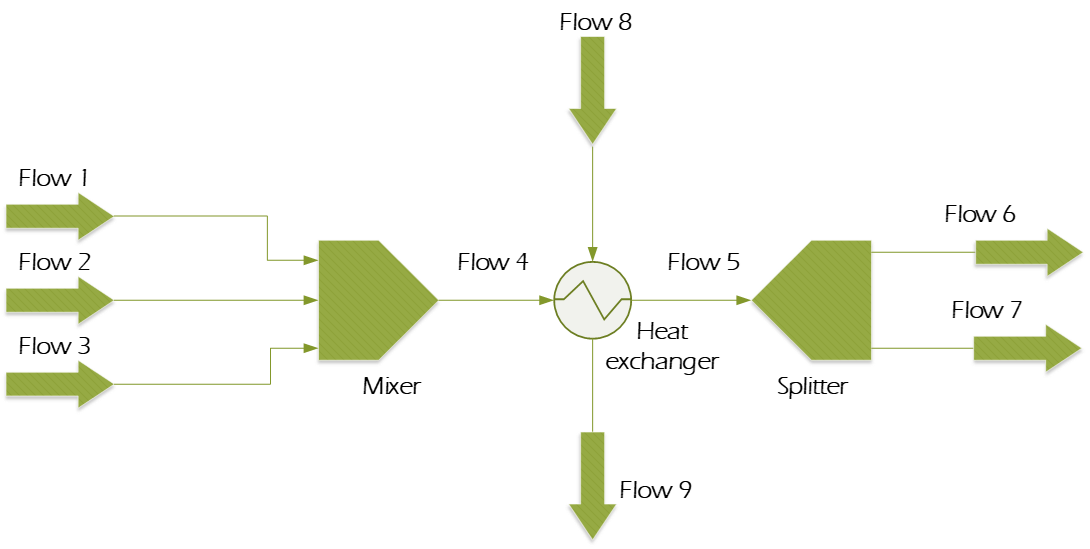
\includegraphics[width=.8\textwidth]{./pics/pfd}
\end{figure}
\vfill
Для решения поставленной задачи будет реализована объектная модель: каждый элемент химико-технологической системы будет описан как отдельный класс.
\vfill
\end{frame}

\subsection{Описание класса \texttt{Flow}}
\begin{frame}[fragile]{Описание класса \texttt{Flow}}
\scriptsize
\begin{table}[h!]
	\centering
	\renewcommand{\arraystretch}{1.2}
	\begin{tabular}{|p{.49\linewidth}|p{.49\linewidth}|}
		\hline
		\textbf{Атрибуты класса} & \textbf{Описание}  \\
		\hline
		\mintinline{python}|mass_flow_rate: float| & Массовый расход, кг / ч \\
		\hline
		\mintinline{python}|mole_flow_rate: float| & Мольный расход, кмоль / ч \\
		\hline
		\mintinline{python}|volume_flow_rate: float| & Объемный расход, м$^3$ / ч \\
		\hline
		\mintinline{python}|mass_fractions: np.ndarray| & Массовые доли \\
		\hline
		\mintinline{python}|mole_fractions: np.ndarray| & Мольные доли \\
		\hline
		\mintinline{python}|volume_fractions: np.ndarray| & Объемные доли \\
		\hline
		\mintinline{python}|temperature: float| & Температура потока, К \\
		\hline
		\mintinline{python}|density: float| & Плотность потока, г / см$^3$ \\
		\hline
		\mintinline{python}|average_mol_mass: float| & Средняя молекулярная масса потока, г / моль \\
		\hline
		\mintinline{python}|cp: float| & Массовая теплоемкость потока, кДж / кг \\
		\hline
\begin{minipage}{\linewidth}
\begin{minted}[frame=none, linenos=false]{python}
def __init__(
    self,
    mass_flow_rate: float,
    mass_fractions: np.ndarray,
    temperature: float
) -> None
\end{minted}
\end{minipage}
		& Создает новый экземпляр класса \texttt{Flow}, заполняя все поля \\
		\hline
	\end{tabular}
\end{table}
\vfill
\end{frame}

\subsection{Функции для пересчета составов}
\begin{frame}[fragile]{Функции для пересчета составов}
\scriptsize
\begin{enumerate}
\item Пересчет массовых долей в объемные:
\vfill
\begin{equation*}
	\varphi _i = \dfrac{\dfrac{\omega _i}{\rho _i}}{\sum \limits _{i=1}^{n} \dfrac{\omega _i}{\rho _i}}
\end{equation*}
\vfill
где $\varphi _i$~-- объемная доля $i$-го компонента; $\omega _i$~-- массовая доля $i$-го компонента; $\rho _i$~-- плотность $i$-го компонента; $n$~-- число компонентов в системе; $i$~-- индекс компонента в системе.
\vfill
\item Пересчет массовых долей в мольные:
\vfill
$$
	\chi _i = \dfrac{\dfrac{\omega _i}{M_i}}{\sum \limits_{i=1}^{n}\dfrac{\omega _i}{M_i}}
$$
\vfill
где $\chi _i$~-- мольная доля $i$-го компонента; $\omega _i$~-- массовая доля $i$-го компонента; $M_i$~-- молярная масса $i$-го компонента; $n$~-- число компонентов в системе; $i$~-- индекс компонента в системе.
\vfill
\end{enumerate}
\vfill
\end{frame}


\subsection{Функции для расчета плотности  и средней \\ молекулярной массы}
\begin{frame}[fragile]{Функции для расчета плотности и средней \\ молекулярной массы}
\scriptsize
\begin{enumerate}
\item Расчет плотности:
\vfill
\begin{equation*}
	\rho = \dfrac{1}{\sum \limits_{i=1}^{n}\dfrac{\omega_i}{\rho_i}}
\end{equation*}
\vfill
где $\rho$~-- плотность потока; $\omega _i$~-- массовая доля $i$-го компонента; $\rho _i$~-- плотность $i$-го компонента; $n$~-- число компонентов в системе; $i$~-- индекс компонента в системе.
\vfill
\item Расчет средней молекулярной массы потока:
\vfill
$$
	m = \dfrac{1}{\sum \limits_{i=1}^{n}\dfrac{\omega_i}{M_i}}
$$
\vfill
где $m$~-- средняя молекулярная масса потока; $\omega _i$~-- массовая доля $i$-го компонента; $M_i$~-- молярная масса $i$-го компонента; $n$~-- число компонентов в системе; $i$~-- индекс компонента в системе.
\vfill
\end{enumerate}
\vfill
\end{frame}

\subsection{Функции для расчета теплоемкости потока}
\begin{frame}[fragile]{Функции для расчета теплоемкости потока}
\scriptsize
Расчет теплоемкости потока в зависимости от состава потока и температуры среды осуществляется следующим образом:
\begin{itemize}
\item определяется теплоемкость компонентов потока при температуре среды:
\vfill
$$
	Cp_i = \sum \limits _{j=1} ^{5} j \cdot k\left[i, j\right] \cdot T^{j-1}
$$
\vfill
где $Cp_i$~-- теплоемкость $i$-го компонента, кДж / кг; $k\left[i, j\right]$~-- коэффициенты аппроксимации температурной зависимости энтальпии для $i$-го компонента; $T$~-- температура потока, К;
\vfill
\item определяется общая теплоемкость потока:
\vfill
$$
	Cp = \sum \limits _{i=1} ^{n} \omega _i \cdot Cp_i
$$
\vfill
где $\omega _i$~-- массовая доля $i$-го компонента; $Cp_i$~-- теплоемкость $i$-го компонента, кДж / кг; $n$~-- число компонентов в системе.
\end{itemize}
\vfill
\end{frame}


\subsection{Описание класса \texttt{Mixer}}
\begin{frame}[fragile]{Описание класса \texttt{Mixer}}
\scriptsize
\begin{table}[h!]
	\centering
	\renewcommand{\arraystretch}{1.2}
	\begin{tabular}{|p{.49\linewidth}|p{.49\linewidth}|}
		\hline
		\textbf{Атрибуты класса} & \textbf{Описание}  \\
		\hline
\begin{minipage}{\linewidth}
\vfill
\begin{minted}[frame=none, linenos=false]{python}
def mix(self, *flows: Flow) -> Flow
\end{minted}
\vfill
\end{minipage}
		& Реализация метода смешения потоков. Возвращает результирующий поток в виде объекта класса \texttt{Flow}\\
		\hline
\begin{minipage}{\linewidth}
\vfill
\begin{minted}[frame=none, linenos=false]{python}
def __calculate_temperature(self) -> float
\end{minted}
\vfill
\end{minipage}
		& Закрытый метод, необходимый для расчета температуры смесевого потока \\
		\hline
	\end{tabular}
\end{table}
\vfill
\end{frame}

\subsection{Материальный и тепловой балансы смешения}
\begin{frame}[fragile]{Материальный и тепловой балансы смешения}
\scriptsize
Состав смесевого потока (в массовых долях) можно найти следующим образом:
\vfill
$$
	\omega _i = \dfrac{\sum \limits_ {j=1} ^{n} G_j \cdot \omega _{i,j}}{\sum \limits_ {j=1} ^{n} G_j}
$$
\vfill
где $\omega _i$~-- массовая доля $i$-го компонента; $G_j$~-- массовый расход $j$-го потока, кг/ч; $\omega _{i,j}$~-- массовая доля $i$-го компонента в $j$-ом потоке; $n$~-- количество смешиваемых потоков.
\vfill
Теплоемкость смесевого потока можно найти следующим образом:
\vfill
$$
	Cp = \dfrac{\sum \limits _{i=1} ^{n} G_i \cdot Cp_i}{\sum \limits _{i=1} ^{n} G_i}
$$
\vfill
где $Cp$~-- теплоемкость смесевого потока, кДж/кг $\cdot$ К; $G_i$~-- массовый расход $i$-го потока, кг/ч; $Cp_i$~-- теплоемкость $i$-го потока, кДж/кг $\cdot$ К; $n$~-- количество смешиваемых потоков.
\vfill
\end{frame}

\begin{frame}[fragile]{Материальный и тепловой балансы смешения}
\scriptsize
Температура смесевого потока определяется следующим образом:
\vfill
$$
	T = \dfrac{\sum \limits _{i=1} ^{n} G_i \cdot Cp_i \cdot T_i}{G \cdot Cp\left(T\right)}
$$
\vfill
где $T$~-- температура смесевого потока, К; $G_i$~-- массовый расход $i$-го потока, кг/ч; $Cp_i$~-- теплоемкость $i$-го потока, кДж/кг $\cdot$ К; $n$~-- количество смешиваемых потоков; $G$~-- массовый расход смесевого потока, кг/ч; $Cp\left(T\right)$~-- теплоемкость смесевого потока, кДж/кг $\cdot$ К, являющаяся функцией от температуры.
\vfill
В итоге получаем нелинейное уравнение, корнем которого является искомое значение температуры смесевого потока.
\vfill
\end{frame}

\subsection{Описание класса \texttt{HeatExchanger}}
\begin{frame}[fragile]{Описание класса \texttt{HeatExchanger}}
\scriptsize
Будем рассматривать теплообменник типа <<труба в трубе>>.
\vfill
\begin{table}[h!]
	\centering
	\renewcommand{\arraystretch}{1.2}
	\begin{tabular}{|p{.49\linewidth}|p{.49\linewidth}|}
		\hline
		\textbf{Атрибуты класса} & \textbf{Описание}  \\
		\hline
\begin{minipage}{\linewidth}
\vfill
\begin{minted}[frame=none, linenos=false]{python}
def __init__(
    self,
    d_in: float = .1,
    d_out: float = .25,
    length: float = 3.0,
    k: float = 4900
) -> None
\end{minted}
\vfill
\end{minipage}
		& Конструктор класса \texttt{HeatExchanger}\\
		\hline
\begin{minipage}{\linewidth}
\vfill
\begin{minted}[frame=none, linenos=false]{python}
def calculate(
    self,
    hot: Flow,
    cold: Flow,
    h: float = .01
) -> tuple[Flow]:
\end{minted}
\vfill
\end{minipage}
		& Расчет теплообменного аппарата.

		 В качестве результата возращается объект кортежа, состоящий из двух элементов: горячего и холодного потоков (объекты класса \texttt{Flow})\\
		\hline
	\end{tabular}
\end{table}
\vfill
\end{frame}

\begin{frame}[fragile]{Описание класса \texttt{HeatExchanger}}
\scriptsize
В стационарном режиме уравнения теплового баланса теплообменного аппарата примут следующий вид:
\vfill
\begin{equation*}
\left\{
\begin{aligned}
	\dfrac{dT_h}{dl} &= -\dfrac{k \cdot \pi \cdot d}{v_h \cdot \rho _h \cdot Cp_h} \cdot \left(T_h - T_c\right) \\
	\dfrac{dT_c}{dl} &= \dfrac{k \cdot \pi \cdot d}{v_c \cdot \rho _c \cdot Cp_c} \cdot \left(T_h - T_c\right)
\end{aligned}
\right.
\end{equation*}
\vfill
где $T_h$ и $T_c$~-- температуры горячего и холодного потоков, соответственно, К; $k$~-- коэффициент теплопередачи; $d$~-- диаметр трубы, м; $v_h$ и $v_c$~-- объемные скорости горячего и холодного теплоносителей, c$^{-1}$; $\rho _h$ и $\rho _c$~-- плотности горячего и холодного потоков, кг/м$^3$; $Cp _h$ и $Cp _c$~-- теплоемкости горячего и холодного потоков, кДж/кг $\cdot$ K.
\vfill
С целью упрощения выберем для решения данной системы дифференциальных уравнений метод Эйлера.
\vfill
\end{frame}


\subsection{Описание класса \texttt{Splitter}}
\begin{frame}[fragile]{Описание класса \texttt{Splitter}}
\scriptsize
\vfill
\begin{table}[h!]
	\centering
	\renewcommand{\arraystretch}{1.2}
	\begin{tabular}{|p{.49\linewidth}|p{.49\linewidth}|}
		\hline
		\textbf{Атрибуты класса} & \textbf{Описание}  \\
		\hline
\begin{minipage}{\linewidth}
\vfill
\begin{minted}[frame=none, linenos=false]{python}
def calculate(
    self,
    flow: Flow,
    *ratio: float
) -> list[Flow]:
\end{minted}
\vfill
\end{minipage}
		& Расчет делителя потока; возвращает в качестве результата список объектов \texttt{Flow} \\
		\hline
	\end{tabular}
\end{table}
\vfill
\end{frame}

\contactsframe[\Large \textbf{Благодарю за внимание!}]{


\includegraphics[width=.05\textwidth]{pics/home} \quad Учебный корпус №2, ауд. 136 \\

\includegraphics[width=.05\textwidth]{pics/mail} \quad chuva@tpu.ru \\

\includegraphics[width=.03\textwidth]{pics/tel} \quad +7-962-782-66-15
}

\end{document}

